\ifx\mainfile\undefined
%  ========================================================================
%  Copyright (c) 2006-2011 The University of Washington
%
%  Licensed under the Apache License, Version 2.0 (the "License");
%  you may not use this file except in compliance with the License.
%  You may obtain a copy of the License at
%
%      http://www.apache.org/licenses/LICENSE-2.0
%
%  Unless required by applicable law or agreed to in writing, software
%  distributed under the License is distributed on an "AS IS" BASIS,
%  WITHOUT WARRANTIES OR CONDITIONS OF ANY KIND, either express or implied.
%  See the License for the specific language governing permissions and
%  limitations under the License.
%  ========================================================================
%
 
\documentclass [11pt, twoside] {uwthesis}

\usepackage{color}
\usepackage{url}
\usepackage{amsmath}
\usepackage{amsfonts}
\usepackage[bookmarks,
	hidelinks,
	plainpages=false,
	pdfpagelabels,
	pagebackref=true,
            ]{hyperref}
\renewcommand*{\backref}[1]{}% for backref < 1.33 necessary
\renewcommand*{\backrefalt}[4]{%
  \ifcase #1 %
    (No citations.)%
  \or
    (Cited on page #2.)%
  \else
    (Cited on pages #2.)%
  \fi
}

\newcommand{\biburl}[1]{{\tt<}\url{#1}{\tt>}}

\hypersetup{%
pdfauthor = {Daniel Chaim Halperin},
pdftitle = {Simplifying the Configuration of 802.11 Wireless Networks with Effective SNR},
pdfsubject = {Ph.D. Dissertation},
pdfkeywords = {},
pdfcreator = {University of Washington, Computer Science and Engineering},
pdfproducer = {},
bookmarksopen = {true},
pdfpagelayout = {TwoColumnRight},
}

\usepackage{footnotebackref}
%%%%%%%%%%%%%%%%%%%%%%%%%%%%%%%%%%%%%%%%%%%%%%%%%%%%%%
%%%        Formatting sections                     %%%
%%%%%%%%%%%%%%%%%%%%%%%%%%%%%%%%%%%%%%%%%%%%%%%%%%%%%%
\newcommand{\algref}[1]{Algorithm~\ref{#1}}
\newcommand{\chapref}[1]{Chapter~\ref{#1}}
\renewcommand{\eqref}[1]{Equation~\ref{#1}}
\newcommand{\figref}[1]{Figure~\ref{#1}}
\newcommand{\secref}[1]{\S\ref{#1}}
\newcommand{\tabref}[1]{Table~\ref{#1}}
\newcommand{\heading}[1]{\vspace{4pt}\noindent\textbf{#1}}
\newcommand{\topheading}[1]{\noindent\textbf{#1}}
\newcommand{\noheading}[0]{\vspace{4pt}\noindent}

%%%%%%%%%%%%%%%%%%%%%%%%%%%%%%%%%%%%%%%%%%%%%%%%%%%%%%
%%%        XXX and other warnings                  %%%
%%%%%%%%%%%%%%%%%%%%%%%%%%%%%%%%%%%%%%%%%%%%%%%%%%%%%%
\newcommand{\xxx}[1]{\textit{\color{red}XXX #1}}

%%%%%%%%%%%%%%%%%%%%%%%%%%%%%%%%%%%%%%%%%%%%%%%%%%%%%%
%%%        Units                                   %%%
%%%%%%%%%%%%%%%%%%%%%%%%%%%%%%%%%%%%%%%%%%%%%%%%%%%%%%
\usepackage{xspace}
\newcommand{\unitsep}{\texorpdfstring{\,}{ }}
\def\unit#1{% from: http://www.tex.ac.uk/cgi-bin/texfaq2html?label=csname "Defining a macro from an argument"
  \expandafter\def\csname #1\endcsname{\unitsep\text{#1}\xspace}%
}
\def\varunit#1#2{% from: http://www.tex.ac.uk/cgi-bin/texfaq2html?label=csname "Defining a macro from an argument"
  \expandafter\def\csname #1\endcsname{\unitsep\text{#2}\xspace}%
}
\unit{GHz}
\unit{MHz}
\unit{kHz}
\unit{Gbps}
\unit{Mbps}
\unit{KB}
\unit{dB}
\unit{dBi}
\unit{dBm}
\unit{W}
\unit{mW}
\varunit{uW}{$\mu$W}
\unit{ms}
\varunit{us}{$\mu$s}
\unit{h}
\unit{m}
\unit{s}
\unit{km}
\unit{cm}
\unit{mm}
\varunit{mmsq}{mm$^\text{2}$}
\varunit{insq}{in$^\text{2}$}
\newcommand{\degree}{\ensuremath{^\circ}\xspace}
\newcommand{\degrees}{\degree}
%%%%%%%%%%%%%%%%%%%%%%%%%%%%%%%%%%%%%%%%%%%%%%%%%%%%%%%%%%%%%%%%%%%%%%%%%%%%%%%%%%%%%%
% Euler for math | Palatino for rm | Helvetica for ss | Courier for tt
%
% From: http://www.tug.org/mactex/fonts/LaTeX_Preamble-Font_Choices.html
%%%%%%%%%%%%%%%%%%%%%%%%%%%%%%%%%%%%%%%%%%%%%%%%%%%%%%%%%%%%%%%%%%%%%%%%%%%%%%%%%%%%%%
\renewcommand{\rmdefault}{ppl} % rm
\usepackage[scaled]{helvet} % ss
\usepackage{courier} % tt
\usepackage{eulervm} % a better implementation of the euler package (not in gwTeX)
\normalfont
\usepackage[T1]{fontenc}
%%%%%%%%%%%%%%%%%%%%%%%%%%%%%%%%%%%%%%%%%%%%%%%%%%%%%%%%%%%%%%%%%%%%%%%%%%%%%%%%%%%%%%

%%%%%%%%%%%%%%%%%%%%%%%%%%%%%%%%%%%%%%%%%%%%%%%%%%%%%%
%%%        Figures                                 %%%
%%%%%%%%%%%%%%%%%%%%%%%%%%%%%%%%%%%%%%%%%%%%%%%%%%%%%%
\usepackage{graphicx}
% Caption package both lets you set the spacing between figure and caption
% and also makes the \figref{} point to the right place.
\usepackage[font=bf,aboveskip=6pt,belowskip=-4mm]{caption}
% Allow subfigures, make them bold
\usepackage[bf,BF,small]{subfigure}
% List of figures
\setcounter{lofdepth}{2}  % Print the chapter and sections to the lot

%%%%%%%%%%%%%%%%%%%%%%%%%%%%%%%%%%%%%%%%%%%%%%%%%%%%%%
%%%        Lists with reduced spacing              %%%
%%%%%%%%%%%%%%%%%%%%%%%%%%%%%%%%%%%%%%%%%%%%%%%%%%%%%%
\usepackage{enumitem}

%%%%%%%%%%%%%%%%%%%%%%%%%%%%%%%%%%%%%%%%%%%%%%%%%%%%%%
%%%        Fancy tables                            %%%
%%%%%%%%%%%%%%%%%%%%%%%%%%%%%%%%%%%%%%%%%%%%%%%%%%%%%%
\usepackage{tabulary}
\usepackage{booktabs}

%%%%%%%%%%%%%%%%%%%%%%%%%%%%%%%%%%%%%%%%%%%%%%%%%%%%%%
%%%        Formatting techniques/tools/etc.        %%%
%%%%%%%%%%%%%%%%%%%%%%%%%%%%%%%%%%%%%%%%%%%%%%%%%%%%%%
\newcommand{\term}[1]{\texttt{#1}}

\begin{document}
 
\textpages
\setcounter{chapter}{7} % Set to n-1!
\fi
%%%%%%%%%%%%%%%%%%%%%%%%%%%%%%%%%%

\cleardoublepage
\chapter{Further Applications of Effective SNR}
\label{chap:applications}

The detailed evaluation presented in the previous chapter showed that my Effective SNR model provides good performance when selecting rates for 802.11a/g and 802.11n links, one important application in wireless link configuration. In this chapter, I present an evaluation of the Effective SNR for four wireless configuration problems to further illustrate the broad applicability of my work.

I chose four problems that represent the key applications needed to configure a future wireless network. The first three are selection algorithms for access points, operating channels, and multi-hop paths through networks. These represent the main decisions (beyond rate) that need to be made in flexible topologies such as Wi-Fi Direct networks. The last application is to classify whether a device is mobile, in order to switch between algorithms designed for static vs. mobile links, or to trigger a search for a new, better operating point when the device begins to move. Together these are the building blocks of an automatically-reconfiguring network that provides good performance.

%%%%%%%%%%%%%%%%%%%%%%%%%%%%%%%%%%%%%%%%%%%%%%%%%%%%%%%%%%%%%%%%%%%%%%%%%%%%%%%%%%%%%%%%%%%%%%%%%%%%%%%%%%%%%%%%%%%%%%%%%%%%%%%%%%%%%%%%%
\section{Experimental Methodology}
To understand how well different techniques perform at the applications studied in this chapter, I took comprehensive measurements of both packet delivery and the RF channel in the University of Washington testbed. These data provide the actual ground-truth performance of links in different configurations and also a record of the channel state during the experiments. Using this data, I perform offline simulations of the different algorithms.

\subsection{Dataset}
I measured the links between 24 static devices in my testbed at the University of Washington. The measurements in this chapter were taken 3 years after the measurements used in \chapref{chap:delivery} and \chapref{chap:rate}, and include a different set of devices. In addition to evaluating the applications in question, the results in this chapter will also tell us whether these NICs in practice experience physical degradation that invalidates their in-factory calibration.

I took measurements on all 35 channels, each 20\MHz wide, that the IWL5300 devices support. Of these 35 channels, 11 overlap in the 83\MHz-wide unlicensed 2.4\GHz band, and the remaining 24 non-overlapping channels are spread across three non-contiguous bands between 5.170\GHz and 5.835\GHz. In an experiment, one sender transmits packets with random payloads to 23 receivers. The transmitter sends a total of 2400 packets by interleaving 100 packets from each of the 24 MCS that correspond to 1-, 2-, or 3-stream 802.11n rates. Each receiver uses 3 antennas for spatial diversity and/or spatial multiplexing. I cycled through all transmitters and all channels over the course of a few hours, and took data at night to attempt to minimize the impact of interference.

\subsection{Computing Ground Truth Packet Delivery}
The above measurements included 100 packets for each link, MCS, and channel. From these data, it is straightforward to compute the ground-truth packet reception ratio (PRR) for each of these configurations. Then for each link $\ell$, I compute the Performance ($P$) of that link at each MCS ($m$):
\begin{equation}
	\label{eq:prr_throughput}
	P_{\ell,m} = \frac{R_{\ell,m}}{100} \cdot B(m),
\end{equation}
where $B(m)$ is the raw bitrate of \mcs{$m$}. Note that while this estimate of performance does not take into account MAC-layer effects, the use of packet aggregation in 802.11n means this is a reasonable proxy.

In this chapter, I decouple the ability to make accurate choices at the application-level from the rate selection algorithm needed to realize it. I thus assume an ideal rate selection algorithm that always correctly chooses the fastest MCS:
\begin{equation}
	\label{eq:best_throughput}
	P_\ell = \max_m P_{\ell,m}.
\end{equation}
These data to provide an Optimal baseline against which I compare Packet SNR- and Effective SNR-based application configuration algorithms.

\subsection{Simulating RF Measurement-based Algorihtms}
While measuring the ground truth performance of the link, I sent exhaustive packet probes at all rates, and collected the RSSI and CSI for each correctly received packet. Of course, this collected information would not be available to an algorithm attempting to quickly assess a channel's performance with RF measurements. Instead, these algorithms are given only the RF measurements from the first packet received in order to compute Packet SNR ($\rho$) and Effective SNR ($\rho_\text{eff}$). By using only the first measurement, I emulate the performance that a configuration algorithm would obtain in practice, where it uses only a single probe.

In the next three sections, I use these data to evaluate how well my Effective SNR model can make access point, channel, and path selections in practice. I use a mobile dataset for the last subsection, and describe it therein.
\section{AP selection}\label{sec:esnr_apsel}
In a dense network, a new client may need to select its parent from many available repeaters in addition to the network coordinator. In enterprise AP and Wireless Distribution System networks today, clients typically choose the node whose probe response has the highest SNR\@. (\xxx{though there is heaps of related work doing more complex things.}) In dual-band networks, some devices may prefer a 5\GHz AP with slightly lower SNR, as long as it exceeds a minimum threshold, based on the optimistic assumption that interference is lower in the 5\GHz band. Here, we describe a procedure that uses the Effective SNR to improve this decision process and select a good parent.

Normally, a client scanning for a network cycles through the available channels sends a probe request at the lowest rate (including a single stream and 20\MHz channels), and all APs or repeaters in range respond. We propose that the client instead send multiple probes that use the lowest 6.5\Mbps rate, but vary the number of streams and channel width in decreasing order. In this way, the coordinator and all repeaters that measure CSI from the probes can compute the Effective SNR for the uplink. The probe responses can now include the computed Effective SNR to better inform the client's choice. If the client includes its transmit power level in the probe request (or if the responder makes a conservative estimate), then the responder can combine this information with the CSI measured from the probe to compute the Effective SNR for the downlink. It can then send the probe response at a faster rate than the base rate and reduce the overhead of the probe response.

%%%%%%%%%%%%%%%%%%%%%%%%%%%%%%%%%%%%%%%%%%%%%%%%
\begin{algorithm}[htp]
\caption{\label{alg:ap_sel_basic}\fcall{APSelection($A, s$)}}
\begin{algorithmic}
\STATE $t_{\max}\gets 0\Mbps$
\STATE $a_{\best} \gets \emptyset$
\FORALL{$a \in A$}
\STATE $t \gets \fcall{PredictThroughput($s, a$)}$
\IF{$t > t_{\max}$}
	\STATE $t_{\max} \gets t$
	\STATE $a_{\best} \gets a$
\ENDIF
\RETURN $a_{\best}$
\ENDFOR
\end{algorithmic}
\end{algorithm}
%%%%%%%%%%%%%%%%%%%%%%%%%%%%%%%%%%%%%%%%%%%%%%%%



\subsection{Evaluation methodology}
Compare the following strategies:
\begin{figure}[p]
	\centering
	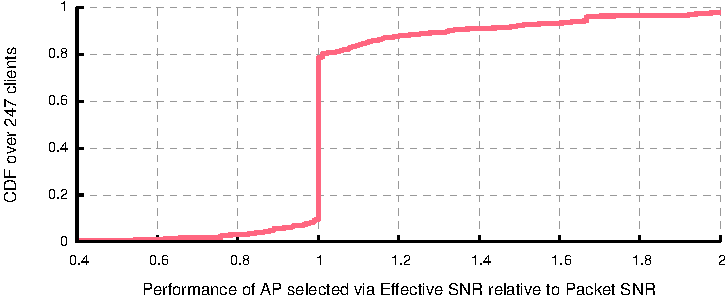
\includegraphics[width=\textwidth]{figures/applications/ap_sel_ratio.pdf}
	\caption{\label{fig:ap_sel_ratio}The relative throughput selecting APs by Packet SNR or by Effective SNR\@.}
\end{figure}

\begin{figure}[p]
	\centering
	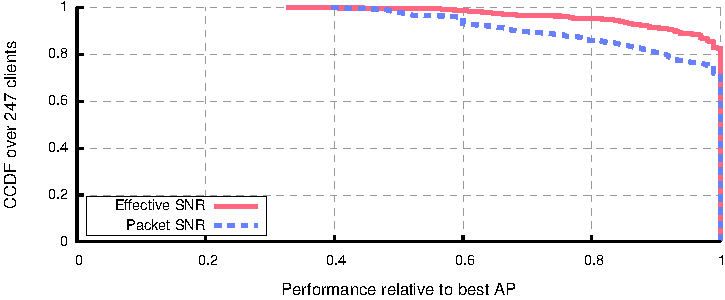
\includegraphics[width=\textwidth]{figures/applications/ap_sel_ratio_opt.pdf}
	\caption{\label{fig:ap_sel_ratio_opt}AP selection using Packet SNR or Effective SNR compared to Optimal.}
\end{figure}

\begin{figure}[p]
	\centering
	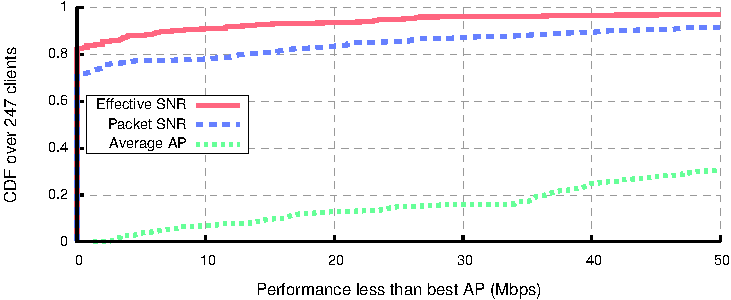
\includegraphics[width=\textwidth]{figures/applications/ap_sel_diff_opt.pdf}
	\caption{\label{fig:ap_sel_delta_opt}The difference in throughput using APs selected by Packet SNR or Effective SNR compared to Optimal.}
\end{figure}
\begin{itemize}
\item first AP seen
\item max RSSI
\item max CSI predicted rate
\item max measured rate
\end{itemize}
%%%%%%%%%%%%%%%%%%%%%%%%%%%%%%%%%%%%%%%%%%%%%%%%%%%%%%%%%%%%%%%%%%%%%%%%%%%%%%%%%%%%%%%%%%%%%%%%%%%%%%%%%%%%%%%%%%%%%%%%%%%%%%%%%%%%%%%%%
\section{Channel Selection}\label{sec:esnr_chansel}
Using the new Wi-Fi Direct standard, 802.11 devices that wish to send data directly (instead of through the access point as in 802.11 infrastructure mode) can create a peer-to-peer link. Depending on the amount of interference in the network (e.g., from other clients of the access point) and the quality of the link between the two devices, they may wish to move the link to a different operating channel in order to improve performance. This is one example of the \emph{channel selection} problem: to quickly choose the best operating frequency for a pair of nodes to communicate. In this section, I define the ``best'' channel to be the channel that provides the highest throughput in the absence of interferers.

The channel selection problem is similar to the access point selection problem, and has a similar algorithmic solution (\algref{alg:chan_sel_basic}). It can use the same \fcall{GetMetric} functions for Packet SNR (\algref{alg:snr_link_metric}) and Effective SNR (\algref{alg:eff_snr_link_metric}). The primary difference is a reordering of the parameters: rather than a fixed receiver with fixed channel choosing between multiple senders, a fixed sender and receiver must choose between multiple channels.

%%%%%%%%%%%%%%%%%%%%%%%%%%%%%%%%%%%%%%%%%%%%%%%%
\begin{algorithm}[thp]
\caption{\label{alg:chan_sel_basic}\fcall{ChannelSelection(Channel Set $C$, Sender $s$, Receiver $r$)}}
\begin{algorithmic}[1]
\FORALL{$c \in C$}
\STATE Both $s$ and $r$ switch to channel $c$
\STATE Compute the channel metric $m_c$ using $\fcall{GetMetric}(s,r)$
\ENDFOR
\RETURN $\argmax_{c\in C} m_c$ \hfill \COMMENT{choose the channel with the best metric}
\end{algorithmic}
\end{algorithm}
%%%%%%%%%%%%%%%%%%%%%%%%%%%%%%%%%%%%%%%%%%%%%%%%

%%%%%%%%%%%%%%%%%%%%%%%%%%%%%%%%%%%%%%%%%%%%%%%%%%%%%%%%%%%%%%%%%%%%%%%%%%%%%%%%%%%%%%%%%%%%%%%%%%%%%%%%%%%%%%%%%%%%%%%%%%%%%%%%%%%%%%%%%
\subsection{Characterization of 802.11 Channels}
To start my investigation of channel selection algorithms, I first measured how the operating frequency affects 802.11n links in practice.

As in \secref{sec:esnr_apsel}, I filtered the data to the 11 channels in the 5\GHz band for which there are not co-channel university APs. (Note that channel selection generally makes sense \emph{within} one frequency band. Selection across bands is trivial: due to better antenna gain and Friis' Law effects a 2.4\GHz channel has typically 10\dB--15\dB stronger SNR than a 5\GHz channel for the same nodes.) I further eliminated from consideration any pairs of devices that didn't obtain at least 6.5\Mbps throughput on at least 3 of the 11 channels. This left 201 unidirectional links, approximately a third of the $24*23=552$ unidirectional links in the testbed.

\begin{figure}[t]
	\centering
	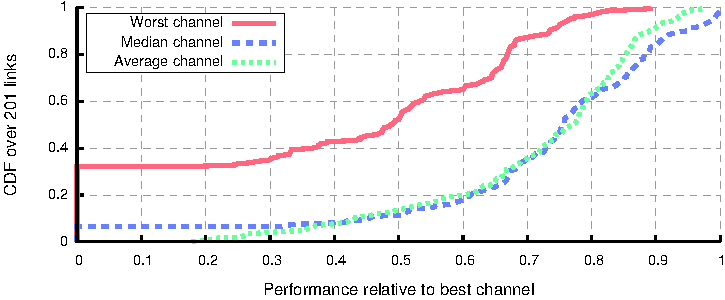
\includegraphics[width=\textwidth]{figures/applications/chan_sel_rel_diff.pdf}
	\caption[The relative difference in throughput over 802.11n channels]{\label{fig:chan_sel_rel_diff}The relative difference in throughput over 802.11n channels.}
\end{figure}

\begin{figure}[t]
	\centering
	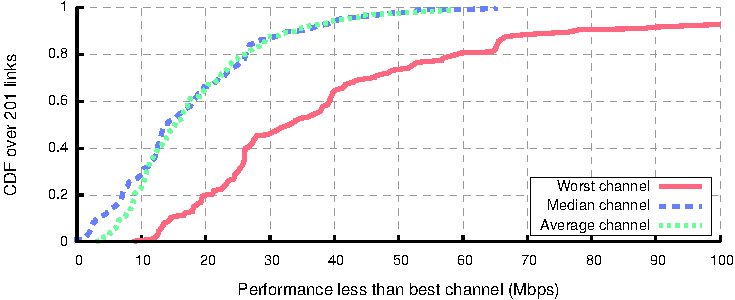
\includegraphics[width=\textwidth]{figures/applications/chan_sel_tpt_diff.pdf}
	\caption[The absolute difference in throughput over 802.11n channels]{\label{fig:chan_sel_tpt_diff}The absolute difference in throughput over 802.11n channels.}
\end{figure}

\subsubsection{Results}
\figref{fig:chan_sel_rel_diff} and \figref{fig:chan_sel_tpt_diff} show how the throughput of the worst, median, and average channels compares to the best channel for these links. Note that because the channel set is fixed and independent of connectivity, the worst channel might deliver no throughput at all---unlike AP selection, in which the client was choosing from only those nodes that responded to its probe. About a third of the links had at least one such channel.

These figures demonstrate that the choice of channel can dramatically impact performance. \figref{fig:chan_sel_rel_diff} shows that the worst channel offers less than half of the best throughput for more than half the links. In absolute terms, this difference can be quite large: the worst channel is a median 33\Mbps worse than the best channel, and for a few links (about 7\%) the difference is more than 100\Mbps. For these links, some channel will deliver no packets at all, while another delivers packets at nearly the maximum bitrate. An unlucky choice of channel can cripple performance and result in little to no throughput.

The median and average channels perform about equivalently in our testbed, and even these are significantly worse. These channels yield less than half the optimal throughput for 15\% of the links and for only one third of links do these come within 80\% of the best throughput. These figures show that for very few links do most channels perform about the same, and the median or average channel is 15\Mbps worse than the best channel for most links, and the gap is larger than 25\Mbps for 20\% of links.

\subsubsection{Signal Strength Across Channels}
Note that the average/median channels are much closer to optimal in these graphs than were the average/median access points we saw in \figref{fig:ap_sel_rel_diff} and \figref{fig:ap_sel_tpt_diff}. Why should this be the case?

I hypothesized that this effect might arise because channels between the same two devices are likely to have similar total signal strengths (i.e., Packet SNR). When two channels have the same signal strength, the difference in performance would come mainly through subchannel fading effects---and while these subchannel effects can affect link quality significantly, as I showed in \chapref{chap:delivery}, the difference is likely not as much as when comparing access points located tens of meters apart.

To test this hypothesis, I analyzed the Packet SNR versus channel for the 11 channels supported by the IWL5300 in the 2.4\GHz band and the 24 channels in the 5\GHz band.\footnote{I used all channels for these experiments, as external interference does not pose a problem. Accurate SNR measurements require only a single packet to be delivered successfully without interference during the preamble.} I considered only links that had at least 10 packets delivered with consistent SNRs and supported at least 3 channels, for a total or 349 links in the 2.4\GHz band and 253 links in the 5\GHz band.

If different channels have similar signal strengths, the Packet SNR will vary only a few dB across the frequency band. \figref{fig:rssi_vs_freq_24} and \figref{fig:rssi_vs_freq_5} plot the normalized Packet SNR for a given link (Packet SNR across all channels minus the average Packet SNR) against channel. The figures include one grey line per link, and the solid black line in each figure shows the median. We see that, indeed, Packet SNR stays within a few dB of the median for most channels. I believe that the shape of the black line in \figref{fig:rssi_vs_freq_5} shows the natural resonance of the antennas, which is consistently non-uniform across the approximately 600\MHz of spectrum the 5\GHz band covers.

\begin{figure}[htp]
	\centering
	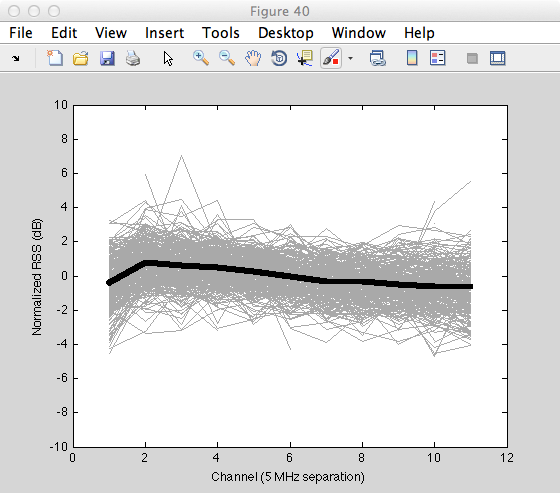
\includegraphics[width=0.6\textwidth]{figures/esnr/rssi_vs_freq_24.png}
	\caption[Normalized Packet SNR versus 2.4\GHz channel for 349 links]{\label{fig:rssi_vs_freq_24}Normalized Packet SNR versus 2.4\GHz channel for 349 links. Solid line shows the median for each channel.}
\end{figure}
\begin{figure}[htp]
	\centering
	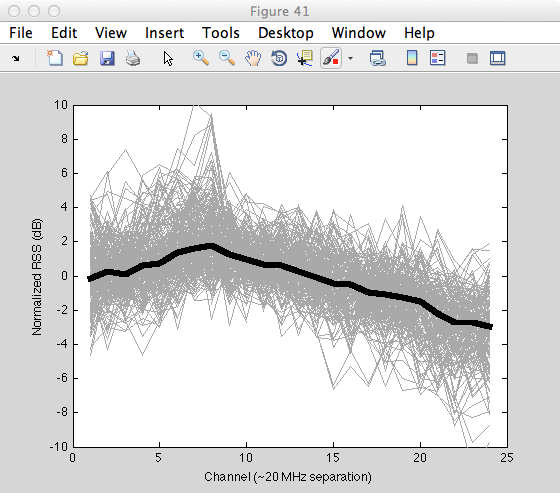
\includegraphics[width=0.6\textwidth]{figures/esnr/rssi_vs_freq_5.png}
	\caption[Normalized Packet SNR versus 5\GHz channel for 253 links]{\label{fig:rssi_vs_freq_5}Normalized Packet SNR versus 5\GHz channel for 253 links. Solid line shows the median for each channel.}
\end{figure}
%\begin{figure}[htp]
%	\centering
%	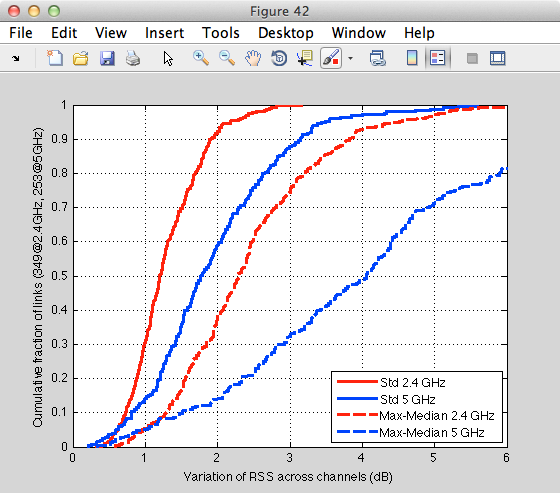
\includegraphics[width=0.6\textwidth]{figures/esnr/rssi_freq_dev.png}
%	\caption{\label{fig:rssi_freq_dev}Standard deviation and max-min spread of Packet SNR across channels within the same band.}
%\end{figure}

From these results, I conclude that a strategy that picks a fixed channel or a random channel will perform significantly worse than a strategy that can identify channels that are likely to offer good performance. Note that this is implicitly the channel selection strategy for strategies that attempt to short-circuit the AP~\cite{Afanasyev_RTSid} used in today's infrastructure networks, because the channel is fixed by the AP. At the same time, because for a fixed link, most channels have roughly the same Packet SNR, fading effects should play a larger role in determining the best channel. This makes the channel selection problem is harder than the AP selection problem, and the solutions may perform slightly worse; however Effective SNR should provide a larger advantage in this case. Having motivated the need for an accurate channel selection algorithm, I present and evaluate different channel selection strategies in the rest of this section.

%%%%%%%%%%%%%%%%%%%%%%%%%%%%%%%%%%%%%%%%%%%%%%%%%%%%%%%%%%%%%%%%%%%%%%%%%%%%%%%%%%%%%%%%%%%%%%%%%%%%%%%%%%%%%%%%%%%%%%%%%%%%%%%%%%%%%%%%%%
%\subsection{Channel Selection Algorithms}
%\algref{alg:chan_sel_basic} is a template for a channel selection algorithm. It takes as input a list of channels to evaluate $C$, and a sender $s$ and receiver $r$ that together define a link. The two nodes hop across channels, using the \fcall{PredictThroughput} function to evaluate the performance of the link on each. The algorithm tracks the best performing channel, labeled $c_{\max}$ and returns that value. (\fcall{ChannelSelection} can also return $\emptyset$ if all channels have zero predicted throughput, but we only consider links that can communicate on at least 1 channel.) Using this template, different channel selection algorithms can be instantiated by providing different implementations of \fcall{PredictThroughput}.
%
%%%%%%%%%%%%%%%%%%%%%%%%%%%%%%%%%%%%%%%%%%%%%%%%%
%\begin{algorithm}[htp]
%\caption{\label{alg:chan_sel_basic}\fcall{ChannelSelection($C, s, r$)}}
%\begin{algorithmic}
%\STATE $t_{\max}\gets 0\Mbps$
%\STATE $c_{\text{best}} \gets \emptyset$
%\FORALL{$c \in C$}
%\STATE Both $s$ and $r$ switch to channel $c$
%\STATE $t \gets \fcall{PredictThroughput($s, r$)}$
%\IF{$t > t_{\max}$}
%	\STATE $t_{\max} \gets t$
%	\STATE $c_{\text{best}} \gets c$
%\ENDIF
%\STATE \textbf{return} $c_{\text{best}}$
%\ENDFOR
%\end{algorithmic}
%\end{algorithm}
%%%%%%%%%%%%%%%%%%%%%%%%%%%%%%%%%%%%%%%%%%%%%%%%%
%
%I consider three different channel selection algorithms in this section. The first is \fcall{ChannelSelectionOPT}, an oracular channel selection algorithm that chooses the optimal channel. For implementation purposes, I instantiate \fcall{ChannelSelectionOPT} by \algref{alg:chan_sel_probe} (\fcall{ProbeChannelThroughput}), which probes all MCSes with MTU-sized packets to determine packet delivery and predicts throughput according to \eqref{eq:prr_throughput}.
%
%%%%%%%%%%%%%%%%%%%%%%%%%%%%%%%%%%%%%%%%%%%%%%%%%
%\begin{algorithm}[tp]
%\caption{\label{alg:chan_sel_probe}\fcall{ProbeThroughput($s, r$)}}
%\begin{algorithmic}
%\STATE $p_0,p_1,\dots,p_{23} \gets 0$
%\STATE $N \gets \text{number of probes at each MCS}$
%\FOR{$i = 1 \dots N$}
%\FOR{$m = 0 \dots 23$}
%\STATE $s$ sends one MTU-sized packet at \mcs{$m$}
%\IF{$s$ receives an ACK from $r$}
%\STATE $p_m \gets p_m + 1$
%\ENDIF
%\ENDFOR
%\ENDFOR
%\STATE $t_{\max}\gets \max \{p_m/N \cdot M(m)\} \text{ over all } m$ \hfill \COMMENT{\eqref{eq:prr_throughput}}
%\STATE \textbf{return} $t_{\max}$
%\end{algorithmic}
%\end{algorithm}
%%%%%%%%%%%%%%%%%%%%%%%%%%%%%%%%%%%%%%%%%%%%%%%%%
%%%%%%%%%%%%%%%%%%%%%%%%%%%%%%%%%%%%%%%%%%%%%%%%%
%\begin{algorithm}[tp]
%\caption{\label{alg:chan_sel_esnr}\fcall{PredictThroughputESNR($s, r$)}}
%\begin{algorithmic}
%\FOR{$m \in \{16, 8, 0\}$}
%\STATE $s$ sends one packet with 0-byte payload at \mcs{$m$}
%\STATE $r$ computes the Effective SNR values $\rho_\text{eff}$ and returns them along with the ACK
%\IF{$s$ receives an ACK from $r$}
%	\STATE \textbf{return} \fcall{ESNRToThroughput}($\rho_\text{eff}$), $\rho_\text{eff}$ \hfill \COMMENT{$\rho_\text{eff}$ is used to break ties}
%\ENDIF
%\ENDFOR
%\STATE \textbf{return} 0
%\end{algorithmic}
%\end{algorithm}
%%%%%%%%%%%%%%%%%%%%%%%%%%%%%%%%%%%%%%%%%%%%%%%%%
%
%The second algorithm chooses the channel based on RSS, presented in \algref{alg:chan_sel_rss}. In this case, the sender only needs to send a single probe packet (with no payload) in order to measure the RSS on the channel. Since \fcall{RSSToThroughput} is monotonically increasing in RSS, this algorithm is equivalent to selecting the channel with the maximum RSS\@.
%
%The third algorithm chooses the channel based on the Effective SNR, presented in \algref{alg:chan_sel_esnr}. Here, the sender sends probes (with no payload) with decreasing numbers of spatial streams to enable the receiver to collect a maximal CSI measurement. The receiver then sends the computed Effective SNR values back to the sender, which uses them to predict the best rate.
%
%I evaluate these three algorithms in the next section.

%%%%%%%%%%%%%%%%%%%%%%%%%%%%%%%%%%%%%%%%%%%%%%%%%%%%%%%%%%%%%%%%%%%%%%%%%%%%%%%%%%%%%%%%%%%%%%%%%%%%%%%%%%%%%%%%%%%%%%%%%%%%%%%%%%%%%%%%%
\subsection{Channel Selection Accuracy}
I evaluate Packet SNR and Effective SNR-based channel selection algorithms based on \algref{alg:chan_sel_basic} and using the link metric functions described in \algref{alg:snr_link_metric} (Packet SNR) and \algref{alg:eff_snr_link_metric} (Effective SNR).

\figref{fig:chan_sel_ratio_opt} shows the performance relative to the optimal algorithm when using Effective SNR or Packet SNR to choose between channels, using the same format as I used for access point selection in \figref{fig:ap_sel_ratio_opt}. Again, we see that both algorithms perform well, though Effective SNR is a better predictor of application performance. Effective SNR chooses an optimal channel for 121 links (60\%), whereas Packet SNR is optimal for only 71 links (35\%). The Effective SNR-based algorithm is within 90\% of optimal for 168 links (84\%), 80\% for 181 links (90\%), and 70\% for 191 links (95\%). In contrast, maximizing the Packet SNR only gets within 90\% of optimal for 112 links (56\%).

\begin{figure}[p]
	\centering
	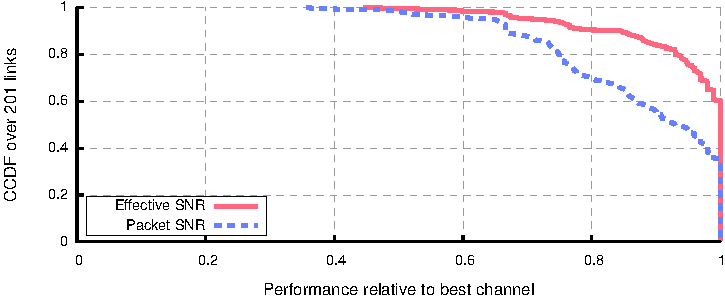
\includegraphics[width=\textwidth]{figures/applications/chan_sel_ratio_opt.pdf}
	\caption[Channel selection algorithm performance relative to Optimal]{\label{fig:chan_sel_ratio_opt}Channel selection algorithm performance relative to an optimal algorithm.}
\end{figure}
\begin{figure}[p]
	\centering
	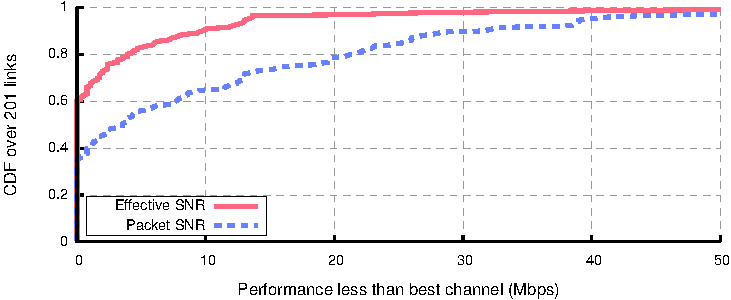
\includegraphics[width=\textwidth]{figures/applications/chan_sel_diff_opt.pdf}
	\caption[Channel selection algorithm performance loss from Optimal]{\label{fig:chan_sel_delta_opt}Channel selection algorithm performance loss from optimal algorithm.}
\end{figure}
\begin{figure}[p]
	\centering
	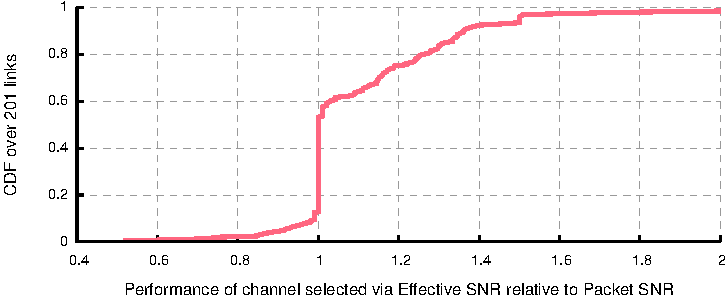
\includegraphics[width=\textwidth]{figures/applications/chan_sel_ratio.pdf}
	\caption[Channel selection algorithm performance with Effective SNR relative to Packet SNR]{\label{fig:chan_sel_ratio}Channel selection performance with Effective SNR relative to Packet SNR.}
\end{figure}

Next, I compare the absolute performance loss of the channel selection algorithms in \figref{fig:chan_sel_delta_opt}. Again, the area over the curves represents the performance lost by each algorithm. This area is 3.3$\times$ larger for the Packet SNR-based selection algorithm, showing that Effective SNR is significantly more accurate. This difference translates to about 9\Mbps faster links when selecting channels via the Effective SNR.

Finally, \figref{fig:chan_sel_ratio} shows the ratio of the performance of the channels selected by Effective SNR and Packet SNR. Recall that a ratio larger than 1 means that Effective SNR chose a faster operating channel. The algorithms choose channels with equal performance for 82 (41\%) of the 201 links, while the Effective SNR-based algorithm chooses a better channel for 94 (47\%) links and the Packet SNR-based algorithm for the remaining 25 (12\%). Additionally, the gains from Effective SNR are much larger than its losses: the Packet SNR strategy chooses a channel that performs 20\% better than the Effective SNR-selected channel for only 4/25 (16\%) links when its channel is better, while Effective SNR chooses a 20\% better channel for 50/94 (53\%) of cases. In other words, the Effective SNR channel selection algorithm is more likely to pick a better channel by a factor of about 4 (94/25), and this difference is more likely to be significant by a factor of about 3 (53\%/16\%).

\heading{Summary.}
These results shows that both Effective SNR- and Packet SNR-based channel selection strategies perform well in my testbed. However, the Effective SNR channel selection strategy is significantly more accurate: it chooses an optimal channel for 70\% more links, it offers about 9\Mbps more per link when selecting suboptimal channels, and it is more likely to choose a better channel than a worse channel by a factor of 4.

Note also that, as hypothesized above, the accuracy of both channel selection algorithms is reduced relative to access point selection. Whereas Effective SNR chose an optimal AP for more than 80\% of clients, it indicates an optimal channel for only 60\% of links; the Packet SNR results exhibit similar a similar decline. This confirms that the similarity of channels leads to more ambiguity when choosing between them. Additionally, the benefits of Effective SNR relative to Packet SNR are larger for channel selection than they were for AP selection. Since most channels have similar Packet SNRs, the real reason for the improvement performance is that my model can accurately assess the impact of subchannel fading effects.

%%%%%%%%%%%%%%%%%%%%%%%%%%%%%%%%%%%%%%%%%%%%%%%%%%%%%%%%%%%%%%%%%%%%%%%%%%%%%%%%%%%%%%%%%%%%%%%%%%%%%%%%%%%%%%%%%%%%%%%%%%%%%%%%%%%%%%%%%%
%\subsection{\xxx{Further Evaluations?}}
%\heading{Channel discrimination.}
%\xxx{how many channels do we need to look at to get good performance?} \figref{fig:rel_diff_draws} shows that, depending on how close to optimal you want to be, need to look at 5, 10, or 15 of the 24 channels in 5\GHz band. If we can evaluate the rate offered by a channel quickly, we can look at more channels in the same amount of time to pick the best rate.
%
%\begin{figure}[htp]
%	\centering
%	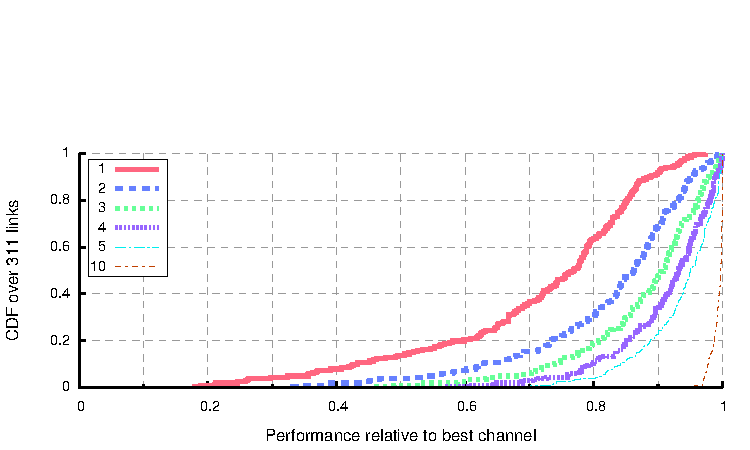
\includegraphics[width=\textwidth]{figures/applications/chan_sel_rel_diff_draws.pdf}
%	\caption[The expected rate after choosing the best of $k$ 802.11n channels]{\label{fig:rel_diff_draws}The expected rate after choosing the best of $k$ 802.11n channels.}
%\end{figure}
%
%\heading{Performance.} \xxx{given time to hop $\mathcal{O}$(1\ms), time to execute a CSI probe $\mathcal{O}$(500\us), and time to execute a rate probe (unknown), how many channels can we look at in $T$ time? Reference \figref{fig:rel_diff_draws} to see what fraction of optimal this enables.}
%
%\heading{Completion Time.} \xxx{The difference between the Effective SNR and the SNR is a proxy for how ``good'' a channel is, based on how flat it is. Given that RSS is similar across channels, the flattest channel will likely offer the best rate. Can we use this to detect a good channel and stop looking early?}
%%%%%%%%%%%%%%%%%%%%%%%%%%%%%%%%%%%%%%%%%%%%%%%%%%%%%%%%%%%%%%%%%%%%%%%%%%%%%%%%%%%%%%%%%%%%%%%%%%%%%%%%%%%%%%%%%%%%%%%%%%%%%%%%%%%%%%%%%
\section{Path selection}\label{sec:esnr_pathsel}
While today's access point and wireless distribution system (WDS) infrastructure networks use tree-structured topologies and have only a single path between any two nodes, a future device-to-device wireless network such as Wi-Fi Direct may offer many paths along which packets can be routed. Choosing which path in a multi-hop wireless network will provide the best throughput is the \define{path selection} problem, and it can be thought of as a generalization of the access point selection problem I described in \secref{sec:esnr_apsel}. Indeed, a client implicitly makes a routing decision when joining a WDS network---which access point it chooses can make a large difference in its connection quality to the root access point that serves Internet access. Research in multi-hop routing for wireless mesh networks~\cite{Bahl_repeater,Rodrig_thesis} has shown that the choice of path can effect a large difference in connection quality.

The practical state of the art in this area is the recent work by Bahl et al.~\cite{Bahl_repeater} on an opportunistic repeater scheme for 802.11a. In this design, when a client with a strong link detects rate anomaly~\cite{Heusse_RateAnomaly}---that is, that its throughput is hurt by a client with a weak link monopolizing airtime---the strong client evaluates whether relaying that client's packets would improve throughout for both. In certain scenarios, they showed that this could improve aggregate performance of the network by 50\%--200\%.

While this solution is practical and works well, the use of new techniques in 802.11n significantly complicates the picture. First, the scheme of Bahl et al.\ uses a link's RSSI (as a measure of Packet SNR) to select between the 8 available 802.11a rates. In contrast, as I have shown in \chapref{chap:delivery}, Packet SNR does not accurately predict the rate for 802.11n links, nor does it enable devices to choose between different MIMO modes. Second, Bahl et al.\ used a homogenous network of single-antenna 802.11a chipsets; but the set of devices in 802.11n networks will be heterogeneous and support differing numbers of antennas and asymmetric transmit/receive capabilities. While it is not clear how to handle these challenges via the Packet SNR, the Effective SNR offers the ability to overcome them. In this section, I evaluate the ability of Effective SNR to deliver the benefits of opportunistic repeaters in 802.11n networks.

Note that the problem of path selection does not differ significantly from that of AP selection, except that when choosing between repeaters (or a direct link) the entire path must be considered rather than merely the last hop. For simplicity, I assume that the network diameter is small such that pipelining~\cite{Rodrig_thesis} is of limited benefit, and do not consider schemes that forward along multiple unreliable paths such as ExOR~\cite{Biswas_ExOR}. I next describe the basic path selection algorithm I evaluate and characterize the multi-hop paths in my testbed.

%Instead, in this section I focus on how 802.11n and heterogeneous devices change the opportunities available from relaying, and whether Effective SNR delivers these improvements.

\subsection{Path selection algorithm}
%%%%%%%%%%%%%%%%%%%%%%%%%%%%%%%%%%%%%%%%%%%%%%%%
\begin{algorithm}[tp]
\caption{\label{alg:relay_sel_basic}\fcall{RelaySelection(Relay Set $R$, Source $s$, Destination $d$)}}
\begin{algorithmic}[1]
\STATE $t_\text{direct} \gets 1/\fcall{PredictBitrate}(s,d)$ \COMMENT{time to send a bit directly from $s$ to $d$, or $\infty$}
\FORALL {$r \in R$}
\STATE \emph{// time to hop through $r$ is the sum of the times of the two hops}
\STATE $t_{\text{relay},r} \gets 1/\fcall{PredictBitrate}(s,r) + 1/\fcall{PredictBitrate}(r,d)$
\ENDFOR
\STATE $r_\text{opt} \gets \argmin_{r\in R} t_{\text{relay},r}$ \COMMENT{find the optimal relay $r_\text{opt}$ with the shortest path}
\IF {$t_{\text{relay},r_\text{opt}} < t_\text{direct}$}
\RETURN $r_\text{opt}$ \COMMENT{if optimal relay offers a shorter path}
\ELSE
\RETURN $\emptyset$ \COMMENT{if the direct link is best}
\ENDIF
\end{algorithmic}
\end{algorithm}
%%%%%%%%%%%%%%%%%%%%%%%%%%%%%%%%%%%%%%%%%%%%%%%%

I describe a simplified path selection algorithm in \algref{alg:relay_sel_basic}. This \define{relay selection} algorithm only considers paths with a single intermediate node (called a \define{relay}). In step 4, this algorithm computes the \define{expected transmission time (ETT)}~\cite{Draves_ETT} of the multi-hop path as the sum of the time to transfer the packet along each hop. This metric makes the optimistic assumption that there is no protocol overhead, and hence provides an overestimate of actual performance, but lets us compare the ability of Packet SNR and Effective SNR algorithms to inform these choices. To balance this optimism, I only consider paths that provide at least 20\% throughput improvement over a direct link.

Relay selection is only a subset of the full path selection problem, but it is simple and recoups much of the potential gain. I considered all $24*23*11=6072$ source-destination-channel tuples in the UW testbed, where I consider each 5\GHz channel as a different instantiation of the network. Of these 6072 node pairs, 2037 (34\%) have a direct link. Adding in optimal one-hop relays enables a further 2317 (38\%) of node pairs to connect, for a total of 4354 (72\%) connected links. The remaining 1713 (28\%) of node pairs require two relays to connect, and would probably be best helped by switching to the 2.4\GHz band in order to obtain higher SNR and longer links.

How much can relaying help in this testbed? To evaluate this, I calculated the bitrate of the optimal one-hop relay choice. I also computed the bitrate of the optimal path using a modification of \algref{alg:relay_sel_basic} to handle multiple hops. (Note that, because it ignores overheads that increase roughly linear in the number of hops, the path bitrate is even more optimistic than the relay bitrate.)

\begin{figure}[t]
\begin{minipage}{0.48\textwidth}
	\centering
	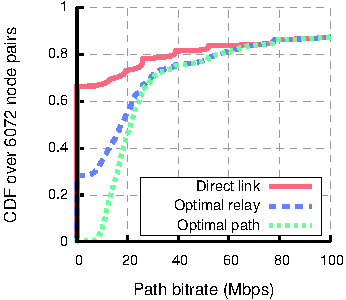
\includegraphics[width=\textwidth]{figures/applications/relay_gains.pdf}
	\caption{\label{fig:relay_sel_gains}Performance of the direct link and the optimal relay or multi-hop path.}
\end{minipage}
\hfill
\begin{minipage}{0.48\textwidth}
	\centering
	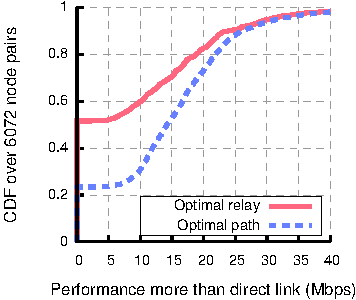
\includegraphics[width=\textwidth]{figures/applications/relay_gains_mbps.pdf}
	\caption{\label{fig:relay_sel_gains_mbps}Performance gain from relay or multi-hop path.}
\end{minipage}
\end{figure}

\figref{fig:relay_sel_gains} shows the net bitrate of the direct link, optimal relay, or best multi-hop path between the 6072 node pairs. This figure demonstrates that the use of a single relay captures most of the improvement for node pairs that can communicate faster than 20\Mbps. Though the relay strategy leaves a quarter of the node pairs disconnected, the optimal multi-hop paths only enable those nodes to communicate at an optimistic estimate of 10--20\Mbps over 3 or more hops. In practice, the benefits to these node pairs would likely be small.

\figref{fig:relay_sel_gains_mbps} shows the achievable improvement in bitrate between the node pairs. Only 25\% (1621/6072) of node pairs gain 20\Mbps or more using these strategies, and 60\% (964) of these also gain 20\Mbps using a single relay.

As these results show that relay selection recoups most of the gains of full path selection in this testbed, I restrict the path selection problem to selecting a good relay for the rest of this section. To complete the description of the algorithms, I now explain how to choose relays using Effective SNR and Packet SNR. To complete \algref{alg:relay_sel_basic}, we need only define the function \fcall{PredictBitrate}, which we use to predict the bitrate of the link studied.

\subsubsection{Relay selection with Effective SNR}
To define the function \fcall{PredictBitrate} for Effective SNR, we can simply use \fcall{GetMetric-EffectiveSNR} (\algref{alg:eff_snr_link_metric})---because the link metric of interest for Effective SNR is indeed simply the predicted bitrate of the link.

\subsubsection{Relay selection with Packet SNR}
Unfortunately, defining a \fcall{PredictBitrate-EffectiveSNR} function for Packet SNR is trickier. We have already seen in \chapref{chap:delivery} that Packet SNR is not a good indicator of packet delivery for a specific MCS, so we can't use the approach we used for Effective SNR in \algref{alg:eff_snr_link_metric}. But there should still be a positively correlated relationship between Packet SNR and expected bitrate, which I use instead to predict the bitrate. (Note that this will not tell \emph{which} specific modulation and coding schemes to use, only what the expected bitrate will be among the many choices.)

\begin{figure}[t]
	\centering
	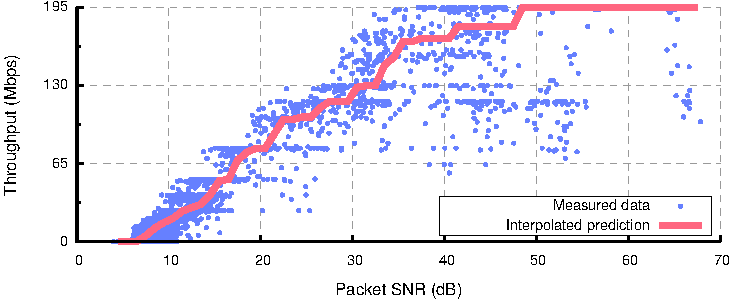
\includegraphics[width=\textwidth]{figures/applications/snr_vs_mbps.pdf}
	\caption{\label{fig:snr_vs_mbps}Deriving a prediction for throughput as a function of Packet SNR.}
\end{figure}

To generate this function, measured the optimal throughput and Packet SNR for all the links in my testbed. I then divided this data into 1\dB-wide SNR bins, and took the median throughput of each bin as the throughput prediction for that Packet SNR value. By connecting these medians (and dropping some sparse bins with so that the line monotonically increases), I derived a monotonic function that uses the Packet SNR measurement to predict the throughput of a link. I plot the original data as a scatterplot in \figref{fig:snr_vs_mbps}, with the interpolated throughput prediction also shown as a solid line. To define \fcall{PredictBitrate-PacketSNR} in order to define a Packet SNR-based relay selection algorithm, I simply look up the Packet SNR of the link and return the throughput predicted by this line.

Having defined both algorithms for relay selection, I next evaluate their performance.

\begin{figure}[t]
	\centering
	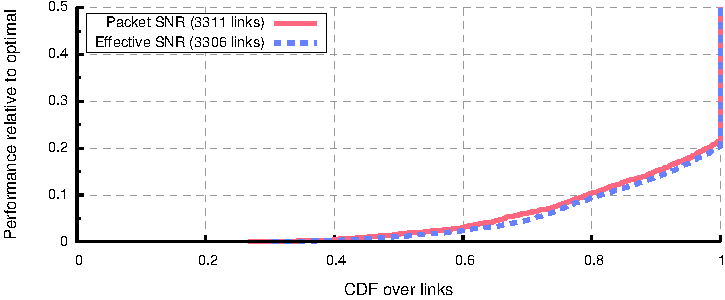
\includegraphics[width=\textwidth]{figures/applications/relay_ratio_opt.pdf}
	\caption{\label{fig:relay_ratio_opt}Relay selection algorithm performance relative to an optimal algorithm.}
\end{figure}
\begin{figure}[t]
	\centering
	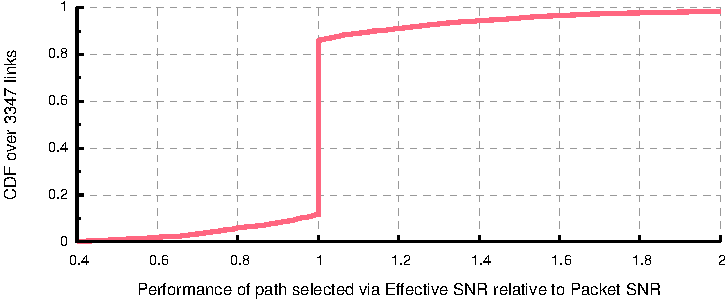
\includegraphics[width=\textwidth]{figures/applications/relay_ratio.pdf}
	\caption{\label{fig:relay_ratio}The relative throughput selecting relays by Packet SNR or by Effective SNR}
\end{figure}

\subsection{Relay selection performance}
I evaluated the performance of \algref{alg:relay_sel_basic} using Packet SNR or Effective SNR to predict performance on the same dataset.

\figref{fig:relay_ratio_opt} plots the relative performance of each algorithm to the optimal relay algorithm, and has a truncated $y$-axis. Note that the algorithms, which choose to use a relay or not based on predictions of performance, do not choose to use a relay for the same number or set of links. Taking the union of the links for which either algorithm chooses a relay, \figref{fig:relay_ratio} shows the ratio of the path chosen using Effective SNR to the path chosen with Packet SNR. Both algorithms perform very well, choosing an optimal relay in 80\% of cases.

The head-to-head comparison shows a potentially surprising result: the Packet SNR and Effective SNR-based algorithms have nearly indistinguishable performance. Effective SNR chooses a better path for 473/3347 (14\%) of links and a worse path for 393 (12\%), but this is a tiny (2.4\%) difference overall. The Effective SNR and Packet SNR lines in \figref{fig:relay_ratio_opt} are nearly indistinguishable. Unlike for access point or channel selection, the ability of Effective SNR to account for subchannel effects does not improve performance over simply using Packet SNR for relay selection.

To explain this phenomenon, recall from \figref{fig:relay_sel_gains} that the links for which performance improves using a relay are those links with low speeds (somewhat less than 100\Mbps). This is because the best possible relay path---a path with two maximum-rate hops (195\Mbps)---would have an idealized rate of 97.5\Mbps. Consequently, direct links that are faster will not benefit from a one-hop relay. Then, these results indicate that the interpolated throughput values in \figref{fig:snr_vs_mbps} are fairly accurate for slower links.

Why would Packet SNR accurately predict the expected performance for slower links? I offer two explanations. First, note that the throughput prediction task that I use to select paths is easier than the packet delivery (\chapref{chap:delivery}) or rate selection problems (\chapref{chap:rate}). Rather than knowing which rate particular configuration points work to provide the best performance, the algorithm need simply predict the expected performance value. This statistical property is easier to get right, and need not be exact in order to find a good path: a slight over- or under-estimate of one or both hops might not change the final path selection. For example, if a hop delivers about 78\Mbps, it does not matter whether this is achieved as \mcs{12} (two streams at 39\Mbps each) or \mcs{19} (three streams at 25\Mbps each). Similarly, for a path using two 78\Mbps hops (total idealized throughput 39\Mbps), an erroneous prediction of 65\Mbps for one hop results in an estimate of 35.5\Mbps which is close to the truth and might still lead to a correct relay selection.

Secondly, slower links are likely to be using single-stream SIMO or dual-stream MIMO2 configurations rather than the three streams used to achieve the absolute fastest rates. The packet delivery results in \chapref{chap:delivery}, particularly as demonstrated by \figref{fig:snr_rate_step_1x3} and \figref{fig:snr_rate_step_2x3}, showed that Packet SNR can be fairly accurate for these configurations, which exploit spatial diversity using the excess receive antennas.

These two factors combined explain why Packet SNR performs well for relay selection in my testbed. This property should generalize, as relaying is generally most useful for slow links. Effective SNR simply offers little gain in this application. Still, Effective SNR performs as well as Packet SNR (if not slightly better) and given its other benefits is a natural fit for this application. %It will also be important in heterogeneous networks where not all relays support the same number of antennas.

%\subsection{Measurements on 802.11a vs 802.11n}
%Denote node in center of testbed as AP, and pick a channel. Consider nodes in decreasing order of RSS: have them associate to the network, then turn into repeaters from which the next node can choose. Assume optimal decisions are made at each step. Compare 1x1, 1x3, and 3x3 versions of this scenario.
%\begin{itemize}
%\item What is the distribution of distance (\#hops) from each node to AP? [How often is repeating used, and at what scale?]
%\item What is the distribution of end-to-end tpt? Of the fraction of max (i.e., 65\Mbps or 195\Mbps)? Of the improvement? [This gets at whether the gains get larger or smaller with various device changes.]
%\end{itemize}
%Same scenario with randomly assigned 3x3, 2x3, and 1x3 devices. How does heterogeneity affect these results?
%
%\subsection{Measurements of Effective SNR}
%Perform the same experiments as described above, this time predicting rate by RSSI and then by Effective SNR\@. (Use this only for topology choice, but assume rate selection finds the correct rate.)
%%%%%%%%%%%%%%%%%%%%%%%%%%%%%%%%%%%%%%%%%%%%%%%%%%%%%%%%%%%%%%%%%%%%%%%%%%%%%%%%%%%%%%%%%%%%%%%%%%%%%%%%%%%%%%%%%%%%%%%%%%%%%%%%%%%%%%%%%
\section{Mobility Classification}\label{sec:esnr_mobility}
The previous three applications in this chapter used the Effective SNR in algorithms that configure various network parameters. In this section, I use the Channel State Information (CSI) underlying the Effective SNR model to determine whether a wireless device is moving. Though this application does not directly use the Effective SNR, this primitive provides an important complement to the network-level configuration problems---in wireless systems, simply knowing whether a device is mobile can improve performance and reliability.

%For example, recent work of Ravindranath et al.\ \cite{Ravindranath_SensorHints} demonstrated a system that improved 802.11a performance on a mobile phone by selecting between different bitrate adaptation algorithms based on whether the device was moving. When the device is static, they use algorithms that can conduct a fine-grained search of the rate space to choose the optimum bitrate. When the device is moving, they use an algorithm that performs a coarser search, but does a better job of tracking a moving optimum. In their experiments, the fine-grained algorithms performed 10\%--30\% better in static scenarios, while the coarse-grained algorithm performed 25\%--75\% better in mobile scenarios.
Detecting mobility can be used to enhance reliability in networks that support dynamic topology, such as today's cellular phone networks, enterprise Wi-Fi wireless distribution systems (WDSes), and networks that support relaying mechanisms such as described above. By proactively looking for a better AP or relay when the device starts moving, service quality can be improved and downtime reduced.
%\xxx{find some references about cell handoff, WDS handoff, etc.}

A recent implementation by Ravindranath et al.~\cite{Ravindranath_SensorHints} detected mobility using the accelerometer in a mobile phone. While this technique is accurate and responsive, it has a few disadvantages. The use of an on-board sensor means that detection can only be performed by the mobile client, and thus requires protocol changes to communicate a device's mobile state to the other endpoint of the link: this solution is not backwards-compatible. Also, this technique can only be implemented on devices that have accelerometers, and requires that this sensor be powered on.

In this section, I explore whether it is possible to classify whether a device is mobile based solely on passively measured RF information. If successful, such an implementation would eliminate all of these drawbacks by requiring no extra hardware and supporting unilateral adoption by either endpoint of the link, including the static device. Ravindranath et al.\ made a preliminary attempt to classify mobility using RSSI, but were not successful. They list three challenges: (1) that RSSI is unstable even for static links in a quiet environment; (2) that RSSI varies by different amounts at different absolute signal strengths, and thus needs to be calibrated; and (3) that RSSI was extremely sensitive to movement in the environment and triggered many false hints. Here, I show that the CSI can overcome these challenges and provide a robust solution.

\subsection{Experimental setup}
I configured a SIMO experiment using a single-antenna laptop as the client device, and eight of the testbed nodes as three-antenna monitors. The client sent 100,000 back-to-back short packets using \mcs{0} (1 stream, 6.5\Mbps), approximately one packet every 200\us for 20\s. This sampling rate is higher than practical for Wi-Fi. In particular, packets sent at slow rates or in batches, can last as long as 4\ms. I thus downsampled the trace from 100,000 packets every 200\us to about 5,000 packets every 4\ms before any of the processing described in the rest of this section.

I ran four experiments to analyze a variety of static and mobile channels. For two experiments, I placed a \emph{static} client in the UW CSE Networking Lab, with students present, but not moving in the room. I next took a trace with \emph{environmental mobility} in which I left the client static, but waved my hand within a few centimeters of the antenna and then walked around the room and opened doors. Finally, I took a \emph{mobile device} trace in which I picked up the laptop and moved it around within a meter of its original location. Chronologically, the traces were taken in the order described within a 10-minute window, with the second static trace taken last.

My goal in this section is to develop a simple classification scheme that can distinguish between these scenarios. In particular, I would like to be able to tell, from RF channel effects alone, whether the device is in a static or mobile channel (with device or environmental mobility). A secondary goal is to distinguish between the two types of mobile channels. Ravindranath et al.\ argued that both of these two goals are difficult, if not impossible, with simple RSSI. I believe that the fine-grained information conveyed by the CSI can overcome these deficiencies.

\subsection{Classifying mobility with RSSI}
I begin by analyzing RSSI variation over time to confirm that it is indeed difficult to distinguish between these four traces. \figref{fig:mobility_rssi} shows the RSSI in dBm measured by one receiver for each scenario. In each plot, the three lines each show the RSSI for one of the three receive antennas. With the typical Wi-Fi noise floor around $-92\dBm$, these graphs show the three antennas for a strong receiver with a Packet SNR around 45\dB.

\begin{figure}[htb]
	\centering
	\subfigure[Static environment]{
		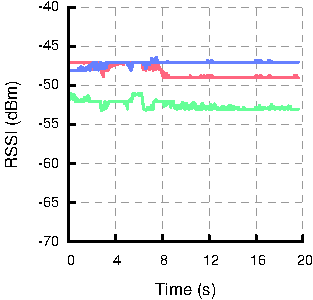
\includegraphics[width=0.43\textwidth]{figures/applications/time_vs_rss_static.pdf}%
	}\hspace{0.06\textwidth}%
	\subfigure[Static environment, trial 2]{
		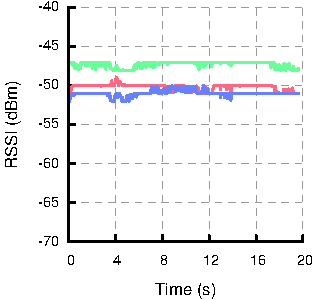
\includegraphics[width=0.43\textwidth]{figures/applications/time_vs_rss_static2.pdf}%
	}
	
	\subfigure[Environmental mobility]{
		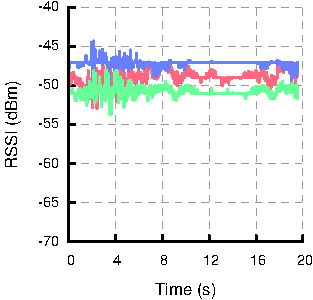
\includegraphics[width=0.43\textwidth]{figures/applications/time_vs_rss_enviro.pdf}%
	}\hspace{0.06\textwidth}%
	\subfigure[Mobile device]{
		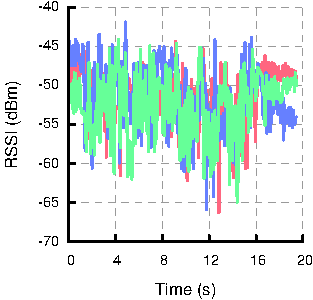
\includegraphics[width=0.43\textwidth]{figures/applications/time_vs_rss_mobile.pdf}%
	}
	\caption[RSSI variation in different mobility scenarios]{\label{fig:mobility_rssi}RSSI variation in different mobility scenarios.}
\end{figure}

I note several interesting effects visible in these measurements. First, the RSSI is actually extremely stable in static scenarios, varying roughly 2\dB across 20 seconds. This stability deviates from the observations by Ravindranath et al., likely because the newer 802.11n hardware I used is well-calibrated, compared with older 802.11g hardware they used to run experiments with the MadWiFi driver.

Second, though RSSI does vary with environmental mobility, the variation is fairly small and mostly limited to the periods of activity directly next to the client. Later in the trace, when I moved across the room, the RSSI variation decreased to match the static scenario. It also appears that the variation is not completely correlated across antennas; in several parts of this trace (e.g., at the beginning and around 10\s--12\s) one or two antennas see variation in RSSI while the others do not. These periods of partial variation may be indicative of a static device with environmental movement.

Finally, the mobile trace exhibits the RSSI variation with the largest magnitude, and shows consistent variation throughout the trace and across all antennas. This is a dramatic outlier compared to the other traces, and strongly reflects the effects of movement.

Based on this visual evidence, which mirrors the results for the other 7 receivers, I believe it likely that the static scenario actually \emph{can} be identified using RSSI, and hypothesize that it may also be possible to distinguish between environmental and device mobility. However, I deferred exploring these possibility further because, as I will show next, the CSI can conclusively classify a device's activity into these three states.

\subsection{Classifying mobility with CSI}
The last subsection examined the four traces I took---two static traces, one with a fixed device and environmental mobility, and the last with a mobile device---and showed that RSSI variation differs visually across in these four scenarios. Here, I examine the same four traces through the lens of the CSI.

\subsubsection{Quantifying CSI variation: Pearson correlation}
Recall that the RSSI yields a single power measurement for each antenna for every packet, whereas the CSI gives a set of matrices of complex numbers that represent magnitude and phase on different spatial paths and frequencies. To measure the deviation in RSSI, we could simply look at its variation---e.g., absolute difference between samples, or windowed variance---over time, as I showed visually in \figref{fig:mobility_rssi}. In contrast, it is not obvious how to quantify the variation in CSI over time.

I chose a simple method to quantify the variation of CSI, by using the \define{Pearson correlation function} for each spatial path between a transmit-receive antenna pair. The Pearson correlation is the ``standard'' correlation for two $n$-element vectors $\vec{x}$ and $\vec{y}$:
\begin{equation}
\textit{corr}(\vec{x},\vec{y}) = \frac{\sum_{i=1}^n(x_i-\overline{x})(y_i-\overline{y})}{\sqrt{\sum_{i=1}^n(x_i-\overline{x})^2 \sum_{i=1}^n(y_i-\overline{y})^2}}.
\end{equation}
Here $\vec{x},\vec{y}$ are indexed by $i$ and have respective means $\overline{x}$ and $\overline{y}$.

To apply this to CSI, let $\vec{r}_{p,t}$ represent the magnitudes of the CSI coefficients across subcarriers for spatial path $p$ at time sample $t$. Then we can quantify the change between sample $t$ and sample $t+1$ by $\textit{corr}(\vec{r}_{p,t},\vec{r}_{p,(t+1)})$. The correlation will be close to 1 if the CSI matches across time, i.e., the channel is not changing, and closer to zero if the channel varies quickly so that the CSI samples are close to being independent.

\begin{figure}[htb]
	\centering
	\subfigure[Static environment]{
		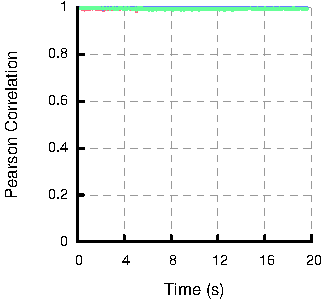
\includegraphics[width=0.43\textwidth]{figures/applications/time_vs_csi_static.pdf}%
	}\hspace{0.06\textwidth}%
	\subfigure[Static environment, trial 2]{
		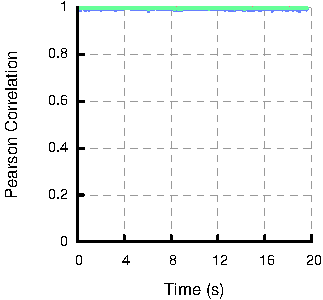
\includegraphics[width=0.43\textwidth]{figures/applications/time_vs_csi_static2.pdf}%
	}
	
	\subfigure[Environmental mobility]{
		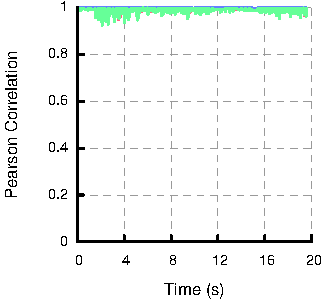
\includegraphics[width=0.43\textwidth]{figures/applications/time_vs_csi_enviro.pdf}%
	}\hspace{0.06\textwidth}%
	\subfigure[Mobile device]{
		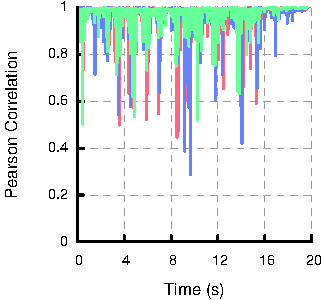
\includegraphics[width=0.43\textwidth]{figures/applications/time_vs_csi_mobile.pdf}%
	}
	\caption[CSI variation as measured by correlation in different mobility scenarios]{\label{fig:mobility_csi}CSI variation as measured by correlation in different mobility scenarios.}
\end{figure}

\subsubsection{CSI variation examples}
Using the same link as in \figref{fig:mobility_rssi}, I present the temporal correlation for the four experiments in \figref{fig:mobility_csi}. Again, each plot shows one line for each of the 3 receive antennas. These plots show that the static traces have near-perfect correlation, close to 1.0 for the full 20\s trace.  In contrast, both the environmental and device mobility traces vary significantly, as low as 0.9 in environmental mobility and 0.3 when the device itself moves. These results thus indicate that the Pearson correlation can classify whether the channel is static, and in changing channel can differentiate whether just the environment is changing or the device itself is moving.

That the environmental and device mobility scenarios exhibit dramatically different correlations might be surprising. To explain this, recall that the frequency-selective channel effects measured by CSI usually result from indoor multipath effects, in which multiple copies of the transmitted signal arrive at the receive antenna after propagating along different (possibly reflected) rays through the RF environment. In many cases of environmental mobility only some of these rays will be affected. If instead the device is itself moving, all paths will be affected. This provides an intuitive explanation for why the temporal correlation is significantly stronger for environmental mobility, though both correlations deviate significantly from the static correlation of 1.

\begin{figure}[tp]
	\centering
	\subfigure[RSSI over time]{
		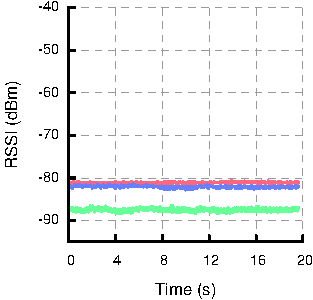
\includegraphics[width=0.45\textwidth]{figures/applications/time_vs_rss_static2_12.pdf}%
	}\hspace{0.03\textwidth}%
	\subfigure[Pearson correlation over time]{
		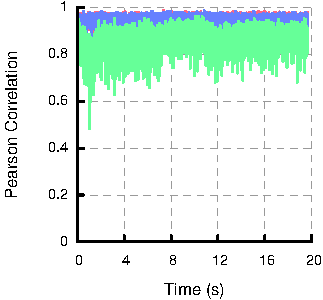
\includegraphics[width=0.45\textwidth]{figures/applications/time_vs_csi_static2_12.pdf}%
	}
	\caption[RSSI and CSI variation for a weak link in a static environment]{\label{fig:mobility_example_weak}RSSI and CSI variation for a weak link in a static environment.}
\end{figure}

\heading{CSI correlation for weak links.}
The Pearson correlation over CSI has thus overcome two of the three drawbacks that Ravindranath et al.\ outlined for classifying mobility using RSSI. First, the correlation of CSI across time is stable for static links. Second, the Pearson correlation can distinguish between environmental mobility and a moving device. The third drawback is that RSSI-based classifiers do not work as well for weaker links: how does my CSI-based classifier perform in this scenario? 

\figref{fig:mobility_example_weak} analyzes the the RSSI and CSI variations during a static trace when the weakest antenna has a Packet SNR of only 5\dB. I found that, indeed, Pearson correlation does not work as well for this weak link. In particular, the correlation against CSI is as low as 0.5, on par with the mobile device for the stronger link shown in \figref{fig:mobility_csi}. The RSSI shown in the left graph also exhibits similarly larger variation for this weak link compared to the strong link analyzed above.

To fix this, I introduced a \define{windowed correlation} scheme. Before computing the Pearson correlation values, I average together 10 consecutive CSI samples. This has the effect of smoothing out the noise corrupting the CSI estimates and restoring the high correlation to the static traces, while only slightly affecting the low correlations for mobile traces.

\begin{figure}[tp]
	\centering
	\subfigure[Windowed CSI correlation for a strong link ($\approx50\dB$ SNR)]{
		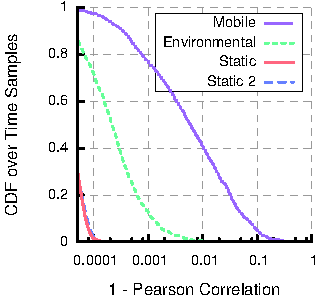
\includegraphics[width=0.45\textwidth]{figures/applications/csi_cdf_link1_10_log.pdf}%
	}\hspace{0.03\textwidth}%
	\subfigure[Windowed CSI correlation for a weak link ($\approx5\dB$ SNR)]{
		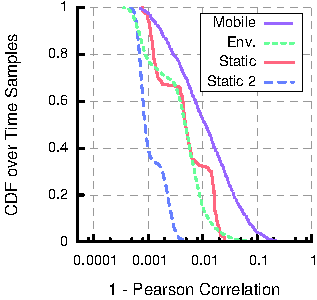
\includegraphics[width=0.45\textwidth]{figures/applications/csi_cdf_link12_10_log.pdf}%
	}
	\caption[Windowed CSI variation for a strong and a weak link]{\label{fig:mobility_csi_cdf}Windowed CSI variation for a strong and a weak link.}
\end{figure}

\figref{fig:mobility_csi_cdf} shows the CDF of the windowed correlation values (denoted $\mathit{corr}$, and combined across antennas) over time for these same two links. To better illustrate the difference across experiments, I capture the deviation from a perfect correlation of 1.0 by plotting $1-\mathit{corr}$ on a logarithmic scale. Thus a value of 0.001 on the $x$-axis means a correlation of 0.999, while a value of 0.1 means a correlation of 0.9. Recall that lower correlations (right on the graph) imply that the channels are changing faster.

For both the weak and the strong link, the mobile trace stands out. Its line to the right, meaning its correlation is lower, than the other measurements for both links. Focusing on the lowest correlations (the points in the bottom 20\% of each CDF), we can see that only the mobile traces achieve a correlation below 0.9 ($x$-axis value 0.1 or higher). For the stronger link, there is clear separation (at least an order of magnitude) between the mobile trace, the environmental mobility trace, and the static traces. For the weak link, it is difficult to distinguish environmental mobility from the static trace. This indicates that the secondary goal of distinguishing these scenarios may only be achievable for strong links.

\subsubsection{CSI correlation results}
Thus far, I have presented CSI correlation results for one strong and one weak link.

The basic mobility classification is as follows. Continually run windowed temporal correlations across CSI measurements for active links, and record the smallest correlation values found. When the smallest correlation is below 0.9 (or over 0.1 in the complementary scale I plot), the classifier will output that the device is mobile. When the largest correlation is below 0.99 (or above 0.01 in the complementary scale), the classifier will output that there may be environmental mobility.

Looking at \figref{fig:mobility_csi_cdf}, we can see that this algorithm will accurately classify mobility, but can result in some static scenarios falsely classified as experiencing environmental mobility. Recall that the traces studied here are 20\,second traces of CSI activity; though only approximately 5\%--20\% of points fall below (above) these thresholds, the peaks are scattered throughout the 20\s trace (e.g., see \figref{fig:mobility_csi}). Over the period at which mobility state can change---at least a few seconds---the classifier should see multiple events.

In \figref{fig:mobility_csi_alllinks_cdf}, I present the CDFs of windowed CSI over all eight links, separated into the three mobility conditions scenarios. Note that the mobility and environmental mobility conditions have 8 lines, one for each receiver, while I have combined both static traces into 16 lines on a single graph. The black vertical lines show the thresholds for environmental mobility (0.01) and device mobility (0.1).

\begin{figure}[htbp]
	\centering
	\subfigure[Mobile device]{
		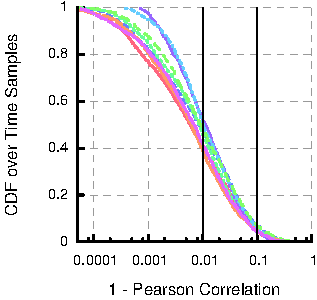
\includegraphics[width=0.3\textwidth]{figures/applications/csi_cdf_mobile_log.pdf}%
	}\hspace{0.03\textwidth}%
	\subfigure[Environmental mobility]{
		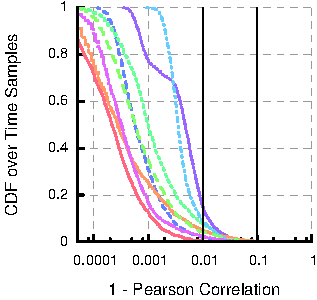
\includegraphics[width=0.3\textwidth]{figures/applications/csi_cdf_enviro_log.pdf}%
	}\hspace{0.03\textwidth}%
	\subfigure[Both static traces]{
		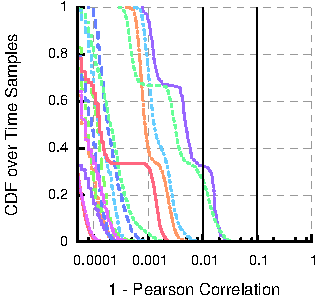
\includegraphics[width=0.3\textwidth]{figures/applications/csi_cdf_static_log.pdf}%
	}
	\caption[Windowed CSI variation for all eight receivers]{\label{fig:mobility_csi_alllinks_cdf}Windowed CSI variation for all eight receivers.}
\end{figure}

These results show that the features I identified looking at the first two links extend to the entire testbed. Notably, all 8 links are properly classified when in device mobility (right of 0.1 on the $x$-axis), while none of the 24 traces in the other two conditions are false positives. For this experiment, my windowed CSI correlation can identify a mobile device across all 8 receivers, some in different rooms and on different floors.

Next, all 8 links are properly classified as being in environmental mobility, with correlations below 0.99 (right of 0.01 on the $x$-axis). Only two static traces reach this level, and those have low Packet SNRs that are near the noise floor. For the combined 16 static traces across the two experiments, most of the links have correlations above 0.999 (left of 0.001 on the $x$-axis) for the entire 20\s period. (Again, the exceptions are the links with very low SNRs.) These latter two figures indicate that windowed CSI correlation can distinguish between static channels and channels with environmental mobility except at very low SNR values.

\subsection{Summary}
The results in this section offer a promising indicators that RF information can indeed provide an accurate classification of device mobility, distinguishing between three different types of RF channels. Though the evaluation is insufficient to prove that these techniques work in all cases, my windowed CSI correlation technique was able to accurately classify device mobility from a static channel for eight different receivers spread across my 802.11n testbed. Additionally, for the 6 of 8 receivers that had strong links, my method could also distinguish between fully static environments and those environments in which people and objects moved near a fixed transmitter.

These results offer evidence that RF measurements can overcome the three drawbacks identified by Ravindranath et al.~\cite{Ravindranath_SensorHints} and provide useful information for mobile system performance. The advantages of an RF-based approach include lower power consumption, compatibility with today's protocols, and the ability for these techniques to be implemented at either end of the link and thus support unmodified legacy devices and devices that do not include sensors.


%In wireless networks today, laptops tend to be ``portable, but not mobile''~\cite{Woodruff_portable}. That is, though they can move from location to location, laptops are infrequently used while actually in motion.


%%%%%%%%%%%%%%%%%%%%%%%%%%%%%%%%%%%%%%%%%%%%%%%%%%%%%%%%%%%%%%%%%%%%%%%%%%%%%%%%%%%%%%%%%%%%%%%%%%%%%%%%%%%%%%%%%%%%%%%%%%%%%%%%%%%%%%%%%
\section{Summary}
In this chapter, I evaluated three algorithms using Effective SNR and one algorithm using Channel State Information to illustrate the flexibility of my model and also flesh out the space of Wi-Fi network configurations. My Effective SNR-based algorithms offer good performance for these applications and make them practical.

Effective SNR provides strong performance improvements over the Packet SNR for the access point and channel selection applications. Interestingly, I found that although Effective SNR can inform multi-hop path selection in the network, it does not perform significantly better than Packet SNR because of the 802.11n spatial diversity techniques that improve the accuracy of Packet SNR.

Finally, inspired by recent work that uses information from onboard sensors to improve link- and network-level performance, I designed and evaluated a pure CSI-based mobility classifier. This classifier can be used to complement the prior applications in a variety of ways, such as informing the nodes in the network when it might be worth looking for a new operating point.

%%%%%%%%%%%%%%%%%%%%%%%%%%%%%%%%%%%%%%%%%%%%%%%%%%%%%%%%%%%%%%%%%%%%%%%%%%%%%%%%%%%%%%%%%%%%%%%%%%%%%%%%%%%%%%%%%%%%%%%%%%%%%%%%%%%%%%%%%

%%%%%%%%%%%%%%%%%%%%%%%%%%%%%%%%%%
\ifx\mainfile\undefined
%
% ==========   Bibliography   ==========
%
%\nocite{*}   % include everything in the uwthesis.bib file
\bibliographystyle{plain}
\bibliography{dhalperi_thesis}

\end{document}
\fi